%!TEX root = ../tommaso-thesis.tex
%!TEX spellcheck = en_US

\definecolor{active}{HTML}{FF6600}
\definecolor{work needed}{HTML}{FF0000}
\definecolor{closed}{HTML}{888888}
\definecolor{resolved}{HTML}{666666}
\definecolor{working on}{HTML}{3388FF}
\definecolor{on hold}{HTML}{55FFFF}
\definecolor{unknown}{HTML}{D3D3D3}


%\chapter{Misery Loves Company:\\CrowdStacking Traces to Aid Problem Detection}\label{ch:stacktraces}
\coolchapter{Misery Loves Company}{CrowdStacking Traces to Aid Problem Detection}{ch:stacktraces}


During software development, exceptions are by no means exceptional: Programmers repeatedly try and test their code to ensure that it works as expected.
While doing so, runtime exceptions are raised, pointing out various issues, such as inappropriate usage of an API, convoluted code, as well as defects.
Such failures result in \emph{stack traces}, lists composed of the sequence of method invocations that led to the interruption of the program.
Stack traces are useful to debug source code, and if shared also enhance the quality of bug reports.
However, they are handled manually and individually, stored in a bug report as a copy-and-paste chunk of text that complicates the automatic processing of the information and raises questions about their reliability.

In this chapter we argue that stack traces can be leveraged automatically and collectively to enable what we call \emph{crowdstacking}, the automated collection of stack traces on the scale of a whole development community.
We present our crowdstacking approach, supported by \slr, a tool which seamlessly collects stack traces during program development and execution and stores them on a central repository.
We illustrate how thousands of stack traces stemming from the IDEs of several developers can be leveraged to identify common \emph{hot spots} in the code that are involved in failures, using this knowledge to retrieve relevant and related bug reports and to provide an effective, instant context of the problem to the developer.

\structure

\secref{sec:stacktraces-intro} outlines the elements involved in collecting runtime information about software errors.
\secref{sec:stacktraces-nature} illustrates the nature of stack traces and describes the data generated during the development process.
\secref{sec:stacktraces-dataset} introduces \slr and the methodology we used to collect stack traces, as well as the process to link them to relevant bug reports.
\secref{sec:stacktraces-evaluation} evaluates our approach.
\secref{sec:stacktraces-discussion} discusses our results.
% \secref{sec:stacktraces-related} analyzes related work on debugging data.
\secref{sec:stacktraces-summary} concludes the chapter and presents the possible extensions to our approach.

\newpage

%%%%%%%%%%%%%%%%%%%%%%
\section{Collecting Runtime Errors} \label{sec:stacktraces-intro}
%%%%%%%%%%%%%%%%%%%%%%

Software development is an iterative refinement process: developers write code and then test it to increase their confidence that the program behaves as desired.
This continuous process of running small, localized tests generates many errors that developers exploit to locate and correct the defects in the code.
Some paradigms, like \emph{Test Driven Development}~\cite{BeckTDD}, adopt an inverse point of view: Developers define tests first, and then write the code that complies with the tests until they all pass.
As a consequence, this process results in an even larger number of runtime exceptions, each of which may contain useful information about the context of failures.

The knowledge enclosed in such exceptions potentially provides useful insights that can be exploited to better understand the underlying system, its functioning, and its quality.
For example, the number and the nature of errors related to the incorrect use of an API is correlated with the difficulty to approach it for a beginner, can suggest a lack of documentation, or a bad architectural design.
Information from exceptions can also be exploited to get a deeper understanding of the runtime behavior of a complex fragment of code, and it is crucial to identify possible defects hidden in the program.

Programming environments generally deal with exceptions by means of \emph{stack traces}, a textual description that depicts the execution of the steps that led to the error.
In object-oriented programming languages this is the sequence of method invocations that led to the exception.

The information in a stack trace is useful to understand where the failure originated and which entities of the system are involved.
Research has shown that it is also valuable to determine the cause of a defect: Including a stack trace in a bug report increases its quality by providing reliable and relevant information.
Indeed, researchers showed that bug reports containing stack traces are closed sooner than bug reports containing only a generic description of the error~\cite{Zimm2010a,Schr2010a}.
However, a stack trace is generally checked manually by a developer to spot and fix single defects and its usefulness terminates once the bug gets resolved.
As a result, a considerable amount of information is discarded and the knowledge it contains is lost.
Researchers already used automated approaches to collect generated stack traces and identify bugs and performance issues~\cite{Glerum2009,Han2012}.
However, these approaches remain \emph{post mortem}, and largely focus on the properties of a running system by recording the behavior of users of operating systems.

We believe that the knowledge contained in stack traces should not be limited to the mere fixing of a single case, and that its use can be extended and in a \emph{live} fashion by automatically and collectively gathering this information, using it to provide instant feedback to the developer.
By establishing such a tight cycle between a failure and the feedback, we want to enable what we call \emph{crowdstacking}, a collective process that involves a whole development community in gathering information automatically collected from stack traces, to boost the debugging process.

We present \slr,\footnote{\url{http://shoreline.inf.usi.ch}} a tool implementing crowdstacking by seamlessly and silently collecting stack traces from development sessions, and storing them on a shared, central repository.
We used the collected data to perform various analyses, such as identifying the entities that are more prone to be involved in a failure, and searching and retrieving relevant knowledge already present in the community ecosystem.
This additional information can be used to prompt a developer during the development process, for example by recommending  a set of bug reports contained in the bug tracker that are related to the current exception, thus providing a more complete picture of the context of the error.



%%%%%%%%%%%%%%%%%%%%%%%%%%%%%%%%%%%%%%%
\section{On the Nature of Stack Traces} \label{sec:stacktraces-nature}
%%%%%%%%%%%%%%%%%%%%%%%%%%%%%%%%%%%%%%%

Exceptions are a common mechanism in modern programming languages to represent errors and signal unexpected behavior in general; they are the standard error management technique in any modern object-oriented programming language.
When they are left unmanaged, and thus they remain uncaught, exceptions ultimately result in the interruption of the executed program.
Normally, an error message gets printed together with a stack trace, which represents the status of the dynamic call stack when the uncaught exception was thrown.
Essentially, it represents a summary of the path that the program followed through the code, showing the entities that were involved before the failure.
We collected large volumes of data from development sessions of users of \pha.
%~\cite{black2009}, an object-oriented programming language  and companion IDE inspired by \textit{Smalltalk}.
In \secref{sec:stacktraces-dataset} we detail the approach we used to collect the stack trace data in the \pha system.


\subsubsection{Anatomy of a Stack Trace}

In \pha, a stack trace is a list of pairs \textit{Class{>}{>}selector}, where \textit{Class} is the name of the class containing the method, and \textit{selector} is the name of the method invoked.
\figref{fig:stacktrace} shows a concrete example of a stack trace that we collected with our tool.

\begin{figure}[ht]
\begin{center}
  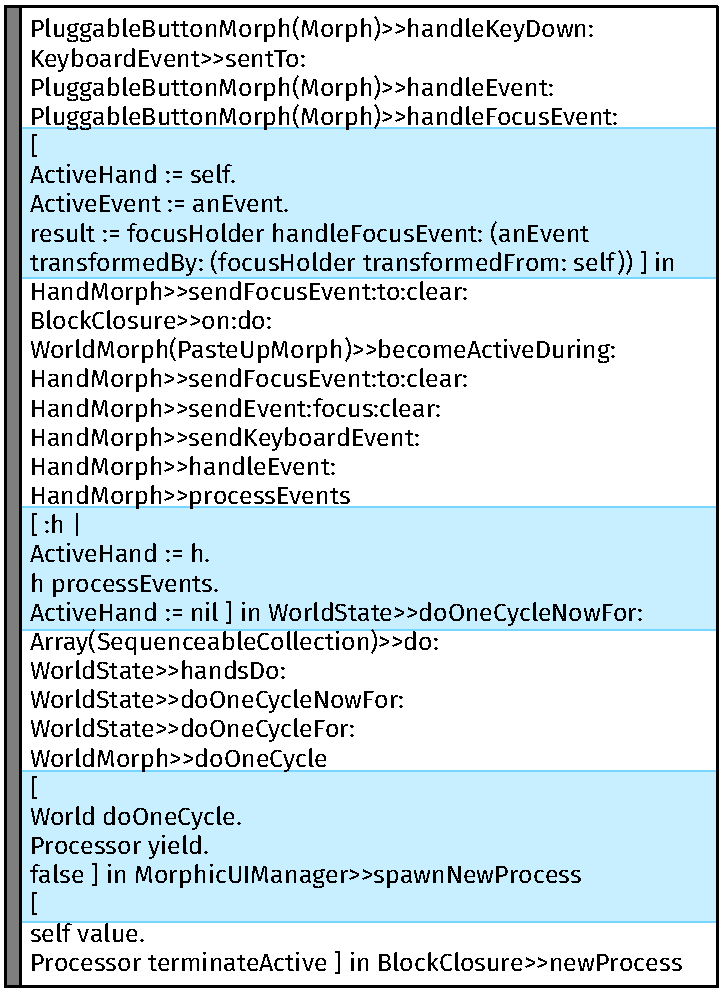
\includegraphics[width=7.3cm]{stacktraces/stacktrace}
  \caption{Example of a stack trace collected from a runtime exception.
The most recent call is at the top, the oldest call is at the bottom.
The snippets of code inside blocks are highlighted in blue.}
  \label{fig:stacktrace}
\end{center}
\end{figure}

As we can see from the listing, the stack trace occasionally contains small snippets of code included in blocks (between square brackets, highlighted in blue).
This happens when a method executes a block.
Since in Smalltalk a block is equivalent to a closure, it represents a pluggable behavior that can change the flow of the program and, as such, it is reported into the stack trace.

Some class names are complemented with the name of a superclass between parenthesis.
This happens when the called method is not defined in the class itself, but it has been inherited from the specified superclass.
This notation maintains the link between the class involved in the exception and its superclass: It is important to keep track of this information, since the cause of an error can be rooted in the superclass chain and suggest a possible defect in the original method, as well as being a consequence of the interaction with the code of the subclass.

\subsubsection{Stack traces and dynamic typing}

An interesting property of \pha comes from its dynamic nature: the whole system is polymorphic, and polymorphism is obtained through the so-called \emph{duck typing}~\cite{Chugh2012}: every object can be used in place of other objects, as long as it is able to respond to the same messages.
This entails that---as in other dynamic programming languages---there is no static type system and, as such, no static type checking: every type error happens at runtime, resulting in a \emph{Message Not Understood} kind of exception.
This peculiarity is important when considering the nature of exceptions in \pha, because the vast majority of the exceptions is caused in this context: In our dataset an exception is thrown as a result of a message not understood in more than 72\% of the cases.
Among those cases, 68\% are generated from a message sent to \emph{UndefinedObject}.
These are the equivalent of a \emph{NullPointerException} in Java.

\begin{figure*}[ht]
\begin{center}
  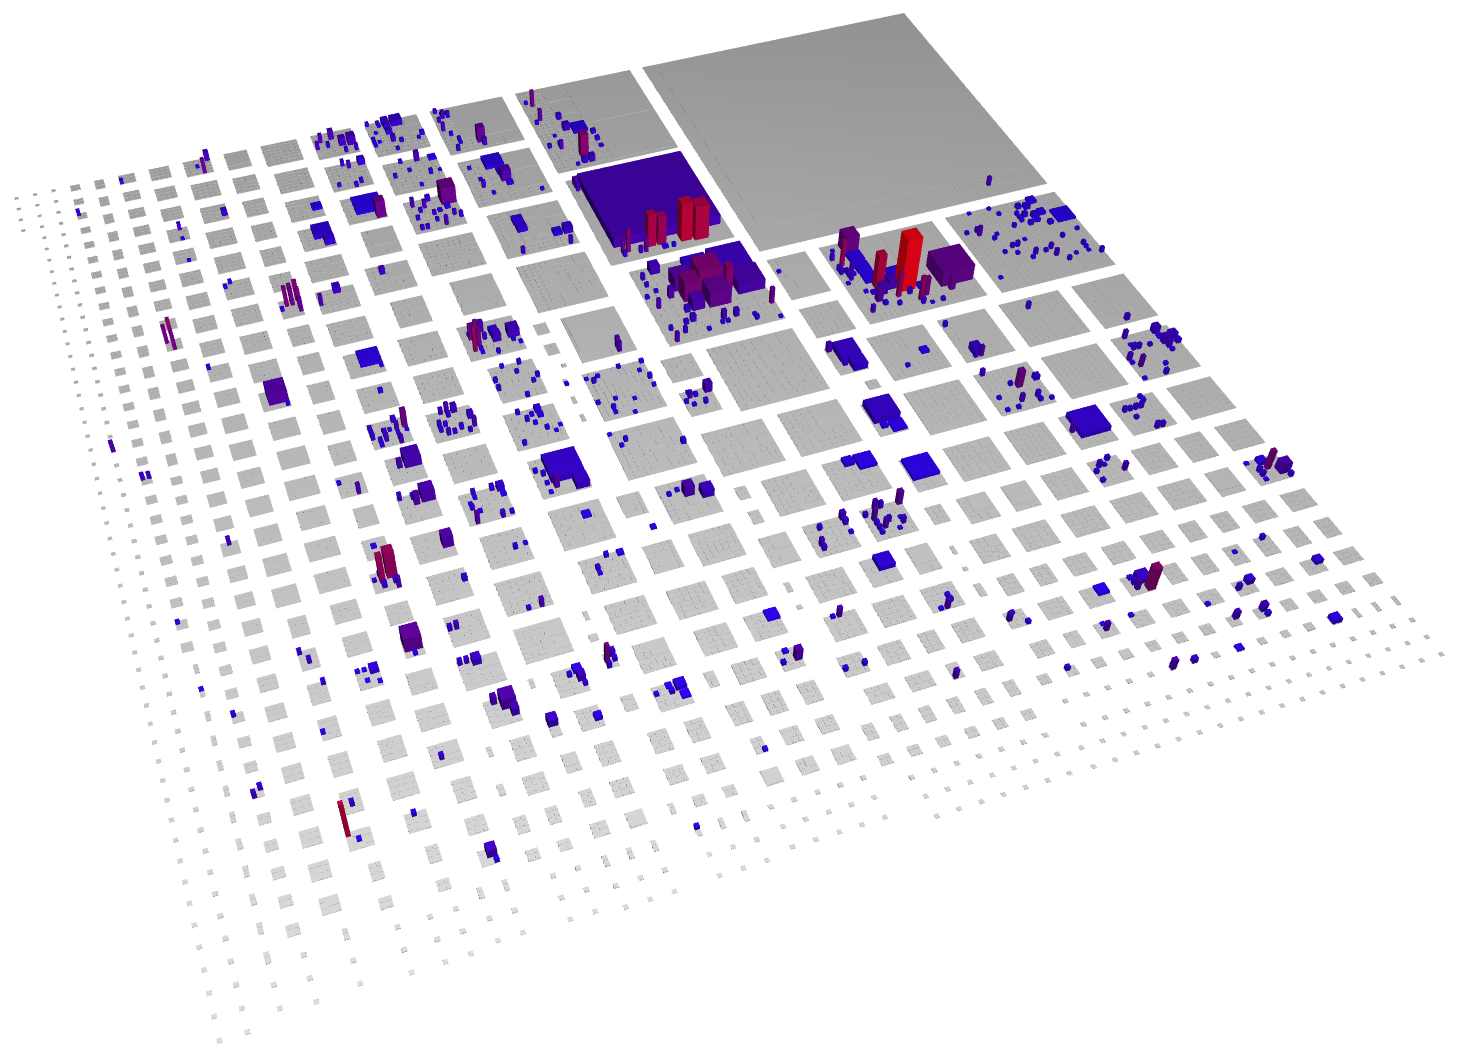
\includegraphics[width=0.9\linewidth,trim=0mm 40mm 0mm 0mm,clip]{stacktraces/StackCity_classes}
  \caption{Distribution of the stack traces on the \pha system using a city like visualization, where each building is a class.
\pha is composed of 14,045 classes distributed among 557 packages.
We highlight the system with data from 7,532 stack traces that we collected.
The height and the color of each building is determined by the number of traces the class appears in, while classes that are not involved in an exception are collapsed and depicted in gray.
The gray squares enclosing the buildings represent the package containing the classes.}
  \label{fig:stackcity-classes}
\end{center}
\end{figure*}

\subsection{Interpreting Stacktraces}

The amount of information represented by type errors is ambivalent: On the one hand, it may be an effect of trivial errors from the user, such as typos, and may represent noise among the useful exceptions.
On the other hand, it contains a large amount of usage knowledge: being able to discriminate the actual failures from the occasional use errors can aid the early identification of defects and speed up debugging.
Also, what at first may look as a ``false positive'', can still be of great help in understanding how users and developers operate the system.
A recurrent and consistent misuse of a method of an API may represent a flaw in the design of the public interface of a library.
The maintainer of the library can then determine how to refactor the interface to improve the documentation.
Moreover, using further data collected after the changes, she would also be able to measure the impact of her intervention on the workflow of the developers.

Another usage example can employ data showing a frequent pattern inside core classes of the system to identify the nodes on the system that manages the largest part of the computation.
By identifying these spots, a developer could be able to prioritize her development activity and to perform targeted optimization.

So far we have considered the \emph{horizontal} dimension of stack traces, that is, we considered the information of a group of traces based on their occurrence.
However, an interesting property that we should also consider is represented by the \emph{vertical} dimension of a stack trace.
Since the order of the elements inside the trace is determined by the call sequence, the depth of a class can give us a hint of the role of the class in the computation: classes near the top of the trace provide an overview of the context where the exception originated, and can therefore be used to provide immediate feedback on the nature of the error and help debugging.
Instead, classes towards the mid part and the bottom of the trace are more related to the mechanics of the system and could be usefully aggregated to identify anomalies in the core parts of the system.

\figref{fig:stackcity-classes} shows the impact that runtime exceptions have on the \pha system, adopting a city visualization~\cite{Wett2011a}.
We aggregated the stack traces in one set of stack calls and counted the number of times a class would appear in a stack trace.
Each class is depicted as a building, where the height and the color represent how often the class is involved in an exception: the more the class appears in a stack trace, the more the color tends to red and the higher the building.
Classes that are not touched by any stack trace are depicted in gray and collapsed.
From this figure we can see how the number of classes involved in exceptions is much lower than the total number of classes in the system, therefore suggesting some hot spots in the system that could be investigated for further development activities.

\subsection{A Practical Use Case}

To be able to deal with a potentially large volume of information, we need an effective approach to classify the stack traces.
In \secref{sec:stacktraces-dataset} we present an approach based on clustering stack traces by similarity, and then stratifying horizontally the clusters using the number of members in each cluster to represent the frequency of the similar exceptions.

The most immediate advantage of using clustered stack traces is to leverage them for bug fixing.
We developed an approach to analyze the contents of a stack trace and use the mined information to retrieve bug reports from the \pha bug tracker that discuss the classes and methods in the trace.
For example, by retrieving the reports related to the trace in \figref{fig:stacktrace}, which involves key events, we can find the bug report $\#12973$, that discusses an issue related to keyboard shortcuts.
By further reading the report, we can learn about the nature of the issue, and by checking the last events we can learn about the current status of the defect.
In this case, we can see that the issue has already been resolved, a patch has been committed and is waiting to be integrated.
Thus, we can ignore the problem, knowing that it will be solved soon.
Moreover, by checking future stack traces, we are able to determine if the problem has been completely solved or if it may appear again in some particular, missed corner cases.

Overall, having quick access to bug reports related to encountered exceptions can help to obtain an overview of the problem and improve and boost the debugging process.
We next discuss how we match bug reports and stack traces.


\section{CrowdStacking Traces}\label{sec:stacktraces-dataset}

Stack traces are a frequent and recurrent side product of the daily workflow of developers.
Such data represent a significant amount of information that is usually not collected and thus lost.
To benefit from this data we built \slr, a tool to intercept exceptions, the corresponding generated stack traces, collect the resulting data and submit it to a central server.


\subsection{Data Collection}\label{sec:stacktraces-tool}

\slr is a plugin designed and built to integrate seamlessly into the \pha development environment.
We wanted to collect unbiased and uniform data, so we posed particular attention in building a tool that could be unobtrusive and that required minimal interaction with the user.
For this purpose, \slr is highly configurable through a dedicated settings menu, and can work in two different main modes: an \emph{interactive mode}, and a \emph{shadow mode}.

\subsubsection{Interactive Mode}
It is designed to allow the developer to keep full control of her data and decide which are the traces to submit and which ones to discard.
\figref{fig:shoreline-reporter} shows the main elements of the interactive user interface.

\begin{figure}[ht]
\begin{center}
  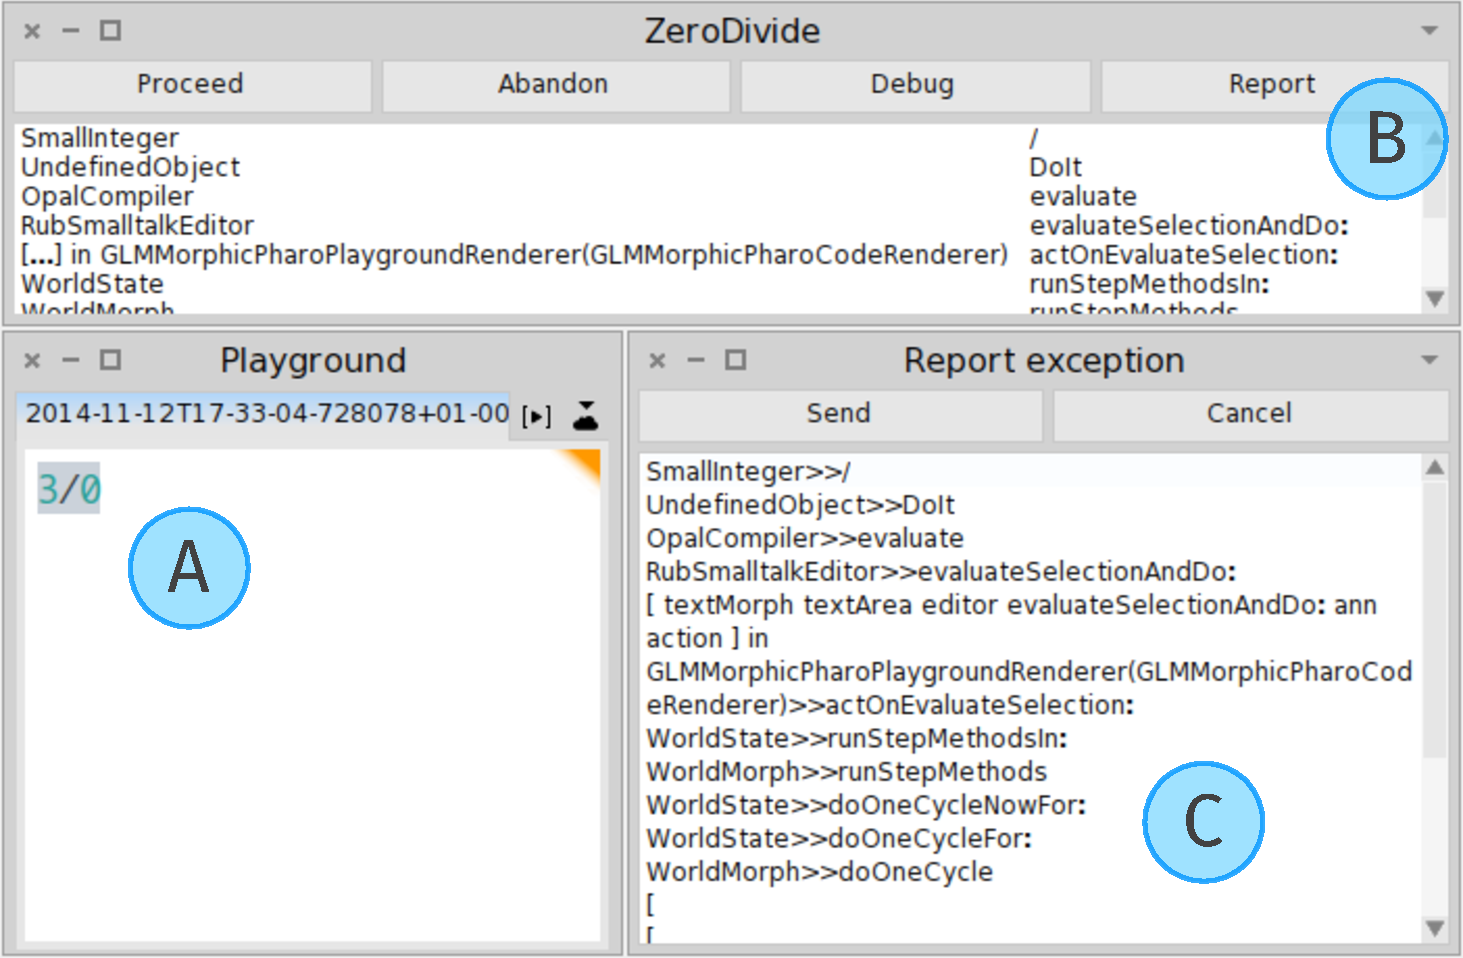
\includegraphics[width=.95\linewidth]{stacktraces/ShoreLine-Reporter.pdf}
  \caption{The interactive interface of ShoreLine Reporter}
  \label{fig:shoreline-reporter}
\end{center}
\end{figure}

\slr activates when the user runs code that triggers an exception \textcircled{\scriptsize A}.
The \pha IDE generally pops up a \emph{pre-debug window} \textcircled{\scriptsize B}, that illustrates a preview of the exception and the options that she can undertake.
Here \slr shows up, proposing a \emph{Report} button that allows the user to send the trace to the ShoreLine server.
If she chooses to do so, she is presented with a window \textcircled{\scriptsize C} that allows her to review the data that is being submitted to verify that it does not leak undesired information.
Once the user presses the \emph{Send} button, the reporter serializes the stack trace and submits it.

\subsubsection{Shadow Mode}
By acting on the system configuration, the user can reduce the level of interaction with the tool at the point of making it become completely transparent: She can decide to submit every stack trace without confirmation and also disable the intermediate check for the data she is sending.
In short, \slr can become completely silent and gather all the stack traces from each exception.
This is particularly important to avoid continuous prompts to the user asking for a confirmation and allow \slr to gather a significant number of stack traces without breaking the workflow of the developer.


\subsection{Data Representation}

In \pha, everything is modeled as an object.
As such, a stack trace is a complex object containing a reference to the debugger, the full context of the exception and the sequence of method calls that constitutes the trace.
However, to value privacy and to avoid our tool from being intrusive, we decided to serialize the whole stack trace as a list of strings, each one containing just the signature of methods, formatted as \textit{ClassName{>}{>}methodSelector}.
Thus, we discard all the elements that contain private data, such as the contents of instance variables.
Encoding a stack trace using strings also guarantees compatibility and portability of the collected data, even when imported from different versions of \pha.

Besides collecting the stack traces, we also added to the report additional metadata to allow a better categorization of the error.
We collect the name of the author, which is the tag she uses to sign her commits, the date of the exception and the version of \pha build for which the exception happened.
The version of the build can be useful to analyze the evolution of the system while it is developed.
The \pha development cycle is structured in two main branches: a stable version and a development version.
In the \pha community, the development version is actively developed and constantly improved by a large number of users and developers, and exception data from developed software can provide insights about the evolution of the system over time, as well as help spotting defects as soon as they arise, ultimately reducing the time required to fix a new defect after it is introduced.

\subsection{Analysis on the Collected Data}

We collected stack traces during a time period of five months, from June to November 2014.
\tabref{tab:data-summary} shows a summary of the data we collected during that time span.

\begin{table}[ht]
\caption{Summary of the stack traces collected from June to November 2014}
\begin{center}
\rowcolors{1}{tablefirstrow}{tablesecondrow}
\begin{tabular}{lr} \hline
\# of stack traces & 7,532 \\
\# of lines in all stack traces & 252,668 \\
\# of developers & 8 \\
average lines of a stack trace & 34 \\
size of the shortest stack trace & 1 \\
size of the longest stack trace & 314 \\ \hline
\end{tabular}
\end{center}
\label{tab:data-summary}
\end{table}

We visualized the data to highlight the parts of the \pha system that were involved in the collected exceptions: \figref{fig:stackcity-methods} shows a city visualization of the stack trace data mapped on the whole \pha system.
Using the same convention used in \figref{fig:stackcity-classes}, each building represents a package and each square enclosing a building is a package.
Each building is composed of blocks, each one representing a method.
The color of each method is determined by the number of times a method appears in a stack trace: it tends to red when the number is higher and to blue when the number is lower.
Methods, classes and packages that do not appear in a stack trace are collapsed and depicted in gray.

\begin{figure}[ht]
\begin{center}
  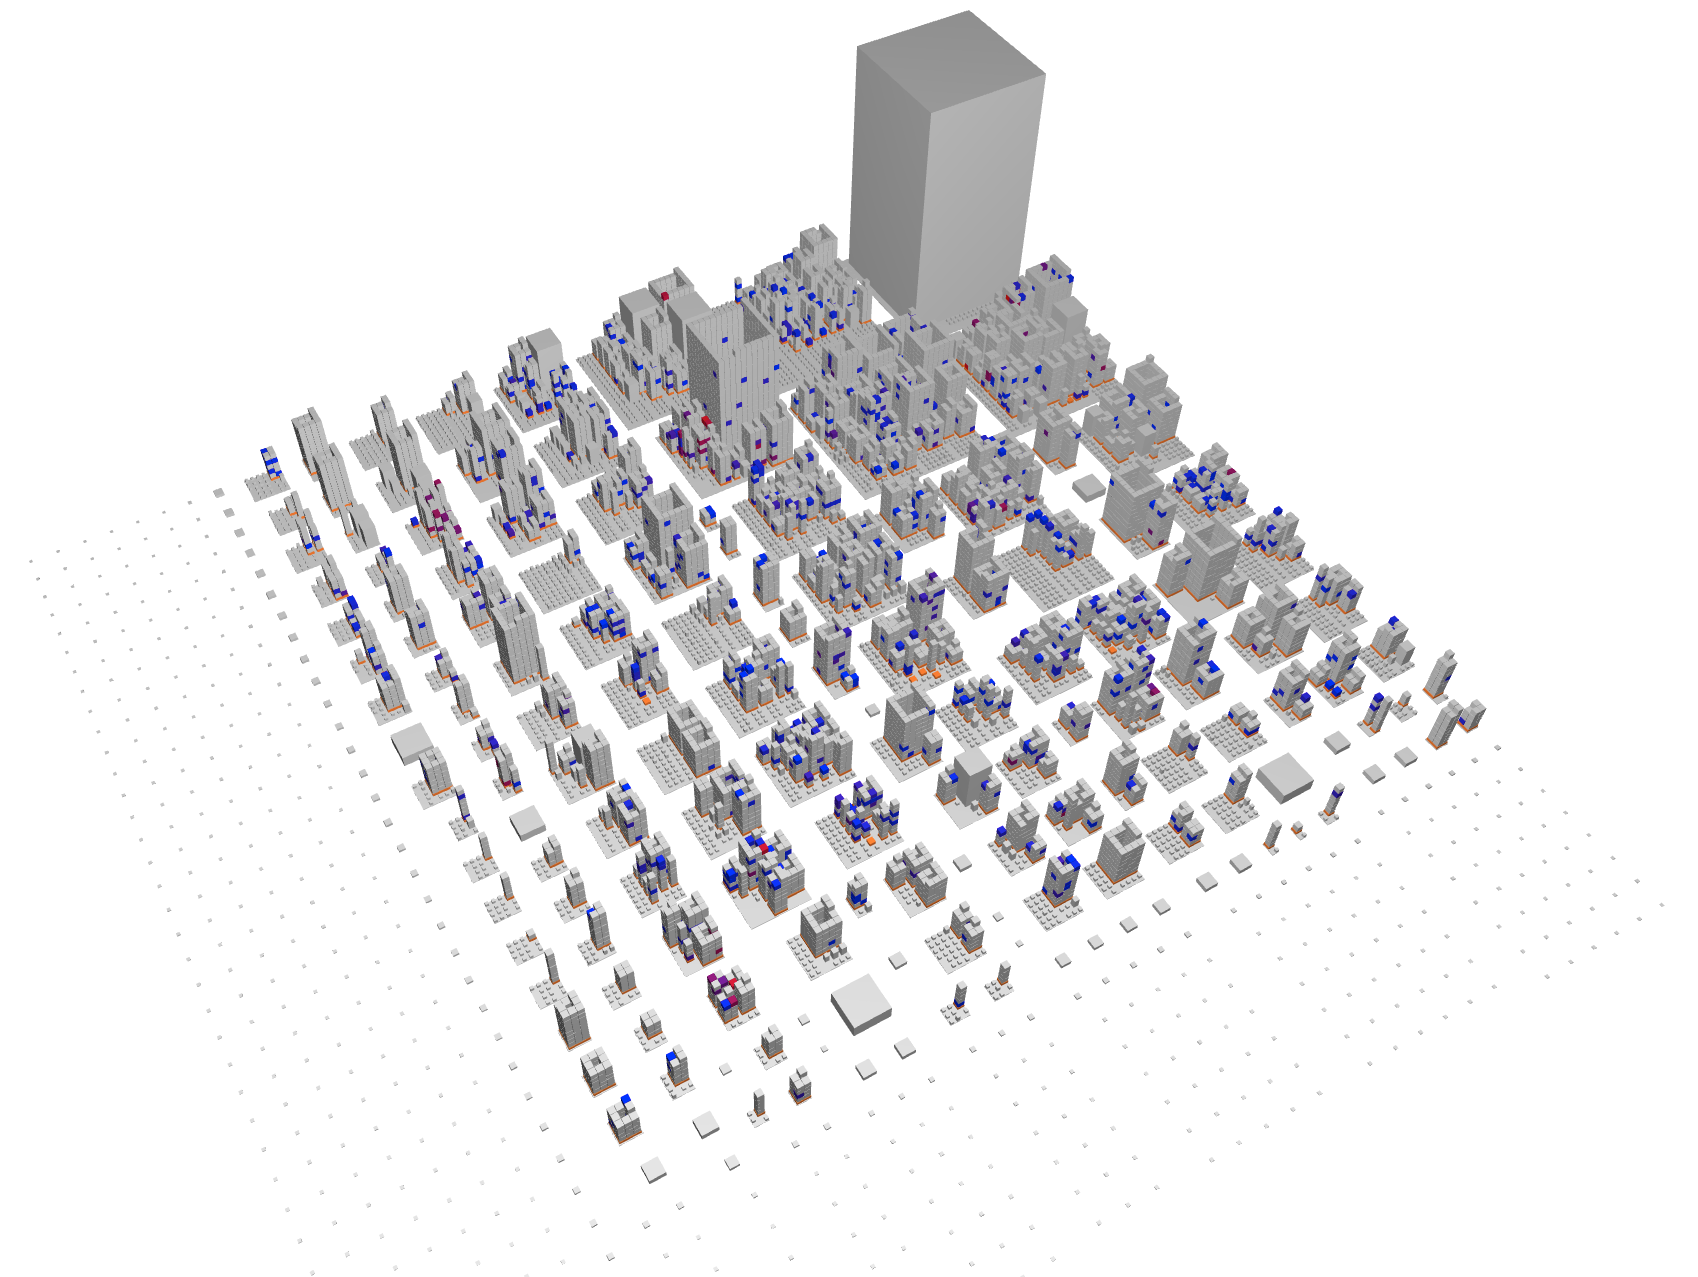
\includegraphics[width=\linewidth,trim=0mm 40mm 0mm 0mm,clip]{stacktraces/StackCity_methods}
  \caption{Distribution of the stack traces on the methods of \pha using a city like visualization, where each building is a class composed by blocks representing methods.
All the classes contain 112,558 methods, the color of each building is determined by the number of traces the class appears in, while the packages, classes and methods that are not involved in an exception are collapsed and depicted in gray.}
  \label{fig:stackcity-methods}
\end{center}
\end{figure}

The figure suggests that only a small part of the system is actually involved in the collected exceptions, and the vast majority of methods and classes is not impacted by these exceptions.
By knowing these methods that work as entry points to the classes, a developer can view the impact that each class and method have in case of failures, and decide which methods she has to inspect first to search for a bug.

\tabref{tab:methods-count} shows a summary of the most active methods in all the stack traces.
\begin{table}[ht]
\caption{The 10 most called methods in the collected stack traces.}
\begin{center}
\rowcolors{1}{tablefirstrow}{tablesecondrow}
\begin{tabular}{lr}
\textbf{Class{>}{>}Method} & \textbf{Occurrences} \\ \hline
BlockClosure{>}{>}on:do: & 9,265 \\
UndefinedObject{>}{>}doesNotUnderstand: & 8,549 \\
BlockClosure{>}{>}cull:cull: & 6,268 \\
Message{>}{>}sentTo: & 4,980 \\
PragmaMenuBuilder{>}{>}collectRegistrations & 4,776 \\
WorldState>>doOneCycleNowFor: & 4,714 \\
BlockClosure>>on:fork: & 4,554 \\
Array>>do: & 4,497 \\
BlockClosure>>ensure: & 4,495 \\
BlockClosure>>cull: & 3,642 \\
%OrderedCollection>>do: & 3,541 \\
%AnnouncementSubscription>>deliver: & 3,490 \\
%BlockClosure>>newProcess & 3,352 \\
%PragmaMenuBuilder>>currentRoot:while: & 3,184 \\
%HandMorph>>sendFocusEvent:to:clear: & 3,078 \\
%WorldState>>doOneCycleFor: & 2,869 \\
%WorldMorph>>doOneCycle & 2,865 \\
%MorphicUIManager>>spawnNewProcess & 2,861 \\
%BlockClosure>>cull:cull:cull: & 2,428 \\
%FormCanvas>>roundCornersOf:during: & 2,017
\hline
\end{tabular}
\end{center}
\label{tab:methods-count}
\end{table}
As expected, the most recurrent exceptions are related to some core elements of the language: \textit{BlockClosure} is a core element used when passing code as argument, while \textit{UndefinedObject>>doesNotUnderstand:} and \textit{Message>>sentTo:} are part of the message sending infrastructure that is the foundation of Smalltalk.
%The former is equivalent to a \textit{NullPointerException} in Java.
Despite being expected, the fact that the most common exceptions involve the dynamic nature of the language shows how the freedom provided by the absence of static type checking comes with the price of incurring in runtime exceptions even for experienced programmers.

Once verified that the most recurring exceptions are caused by common usage patterns of the language, we can consider these elements as outliers for the specific purpose of this work: The information they carry can still be useful in identifying other issues like API usage problems, but it is likely negligible to be connected to bug reports.
Moreover, methods that appear in very few stack traces are also outliers, since there is an intrinsic lack of confidence that they can be significant to represent any pattern in the system.

\subsection{Extracting Information}

We saw that many stack traces are channelled mainly through few crucial points in the system.
To inspect whether it was possible to group them, we applied a clustering approach to detect the stack traces that could be generated by similar errors.
Clustering stack traces can give us the advantage of reducing the number of elements that we have to inspect to determine whether a given error is caused by a defect, by bad usage or simply by a behavior of the developer (\eg in the case of Test Driven Development).
Inspired by a technique used in information retrieval, we mapped our stack traces to a \textit{vector space model}~\cite{salt1975}.
A vector space model is a data structure to index documents and perform efficient comparisons between each document.
In information retrieval it is built by splitting a document in a sequence of terms, and turning the document in a vector counting the number of occurrences of each word in the document.
We build our vector space model by building a vector for each stack trace: we use the pair \textit{ClassName{>}{>}MethodName} to identify the features (the terms) of the vector.
We collected all the features in a dictionary and used it to build each vector, where the components of the vector contain the number of times that a method invocation appears in the stack trace.


For example, consider the two stack traces containing the method calls:
% {\footnotesize
% \begin{center}
% \begin{tabular}{ll}
% \textbf{Trace 1} & \textbf{Trace 2} \\ \hline
% UndefinedObject{>}{>}DoIt & TabManager{>}{>}setTabContentFrom: \\
% BlockClosure{>}{>}valueAfterWaiting: & Tab{>}{>}retrieveMorph: \\
% BlockClosure{>}{>}newProcess & BlockClosure{>}{>}newProcess \\
% \end{tabular}
% \end{center}}
{\footnotesize
\begin{center}
  \begin{tabular}{lll}

    \begin{tabular}{l}
      \textbf{Trace 1} \\ \hline
      UndefinedObject{>}{>}DoIt \\
      BlockClosure{>}{>}valueAfterWaiting: \\
      BlockClosure{>}{>}newProcess \\
    \end{tabular}

    & &

    \begin{tabular}{l}
      \textbf{Trace 2} \\ \hline
      TabManager{>}{>}setTabContentFrom: \\
      Tab{>}{>}retrieveMorph: \\
      BlockClosure{>}{>}newProcess \\
    \end{tabular}

  \end{tabular}
\end{center}}

\pagebreak[2]

We collect all the terms and build a dictionary composed of the features:
{\footnotesize
\begin{center}
\begin{tabular}{l}
\textbf{Dictionary} \\
BlockClosure{>}{>}newProcess \\
BlockClosure{>}{>}valueAfterWaiting: \\
Tab{>}{>}retrieveMorph: \\
TabManager{>}{>}setTabContentFrom: \\
UndefinedObject{>}{>}DoIt
\end{tabular}
\end{center}}

% \begin{stacktrace}
% {\footnotesize
% \begin{center}
% \begin{tabular}{l}
% \textbf{Dictionary} \\
% BlockClosure{>}{>}newProcess \\
% BlockClosure{>}{>}valueAfterWaiting: \\
% Tab{>}{>}retrieveMorph: \\
% TabManager{>}{>}setTabContentFrom: \\
% UndefinedObject{>}{>}DoIt
% \end{center}
% \end{stacktrace}

Using the dictionary we can then build the vectors for the two stack traces:

\begin{center}
\begin{tabular}{p{2cm}r}
\textbf{Trace 1} & $\left<1,1,0,0,1\right>$ \\
\textbf{Trace 2} & $\left<1,0,1,1,0\right>$
\end{tabular}
\end{center}

Once we have our vector space model, we can define the distance between each stack trace.
For this, we need to define a similarity measure, that indicates how two stack traces are different according to our metrics.
Having a vector space model allows us to calculate distances by means of the \emph{cosine similarity}, which for two vectors can be calculated from the definition of the Euclidean dot product, that is:

\begin{displaymath}
    \cos\theta=\frac{A \cdot B}{\|A\|\|B\|}
\end{displaymath}

In the case of documents, where the vectors have all positive components, the similarity ranges from 0 to 1.
In the previous example, the distance for the two vectors representing Trace 1 and Trace 2 is 0.58.
Using the cosine similarity we calculated the first nearest neighbor for each stack trace.
With this data we were able to construct a visualization to understand the topology of the stack traces in our vector space model.

\figref{fig:eva-clusters} shows a force graph where each dot is a stack trace and every edge represents the connection between each trace and its nearest neighbour.

\begin{figure}[h!t]
\begin{center}
  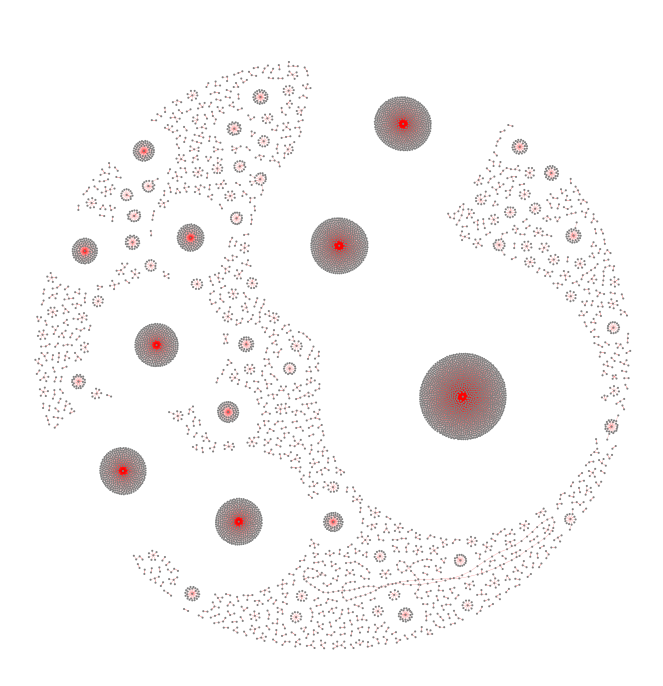
\includegraphics[width=\linewidth]{stacktraces/TraceClusters}
  \caption{Force graph representing the stack traces and their neighbour.
  Each dot is a trace, each edge connects a stack trace with its nearest neighbour.}
  \label{fig:eva-clusters}
\end{center}
\end{figure}

The figure shows evidence that there are groups of related stack traces, gathered around a pivotal point.
In particular, few large groups gather the majority of stack traces, and the remaining form smaller groups.
To represent each cluster, we chose the \emph{medoids}~\cite{Kauf1987}.
A medoid is the element of the dataset that is nearest to the centroid of the cluster.
The advantage of using medoids instead of centroids is that they are element of the dataset, and thus they represent a real occurred stack trace.
Moreover, centroids tend to be much more sparse that medoids, thus being more suitable for efficient computation of operations between vectors.
We considered the medoids as \emph{archetypes}, that represent the summary of each cluster.
The number of incoming edges represents the measure of the popularity of the archetype and, as such, of the whole group.

\begin{table}[ht]
\caption{Summary of the most popular stack traces, with the popularity metrics.}
\begin{center}
\rowcolors{1}{tablefirstrow}{tablesecondrow}
\begin{tabular}{lr}
\rowcolor{tableheader}\textbf{Archetype (first line)} & \textbf{Popularity} \\ \hline
UndefinedObject>>doesNotUnderstand: & 1,585 \\
UndefinedObject>>doesNotUnderstand: & 647 \\
UndefinedObject>>DoIt & 619 \\
UndefinedObject>>doesNotUnderstand: & 428 \\
UndefinedObject>>doesNotUnderstand: & 427 \\
RGFactory>>doesNotUnderstand: & 363 \\
BlockClosure>>doesNotUnderstand: & 127 \\
UndefinedObject>>doesNotUnderstand: & 111 \\
SystemDictionary>>errorKeyNotFound: & 71 \\
MouseWheelEvent>>doesNotUnderstand: & 69 \\
UndefinedObject>>doesNotUnderstand: & 57 \\
NBGLFrameBuffer>>error: & 41 \\
RTDraggable>>initializeElement: & 29 \\
UndefinedObject>>DoIt & 29 \\
UndefinedObject>>DoIt & 28 \\
%R3KeyControl>>initElementForMac: & 28 \\
%R3MouseControl>>initElement: & 26 \\
%UndefinedObject>>doesNotUnderstand: & 26 \\
%SmalllintManifestChecker>>runRules:onPackage:withoutTestCase: & 24 \\
%UndefinedObject>>doesNotUnderstand: & 24 \\
%UndefinedObject>>DoIt & 23 \\
%PluggableButtonMorph>>handleKeyDown: & 23 \\
%SmallInteger>>/ & 18 \\
\hline
\end{tabular}
%\caption{Summary of the most popular stack traces, with the popularity metrics.}
\label{tab:popularity}
\end{center}
\end{table}

From \tabref{tab:popularity} we can see that the largest groups of stack traces are generated by exceptions related to the dynamic nature of the language, and as such probably caused by the style of programming of the developer.
We still believe that this information can provide deep knowledge over the status of the system, but we think that their analysis represents a different set of problems that could be tackled with statistical analysis of big volume of stack traces during the evolution of the system.
Therefore, at this stage we removed the most popular groups, and focused our inspection on the traces positioned in the central part of the ranking.
We used these samples to determine a possible correlation with existing defects.

We mined the \pha bug tracker to collect the bug reports produced during the development of the platform.
To focus our research on actual and relevant problems, but without risking of losing valid examples, we considered the reports opened between January and November 2014.

We extracted 1,910 bug reports, with 17,747 different events, including comments, patches and changes of status.
During this period, 1,591 reports have been closed or are waiting for integration, and 319 are still active.

We then extracted from each archetype of stack trace a list of methods invocation.
We used this list to search through the data extracted from the bug tracker using a full text search of the pair \emph{ClassName{>}{>}MethodName} into the contents of each comment that compose a bug report.
After this operation, we obtained a list of the bug reports that are associated to each method invocation.
Not every bug report can have the same relation with the stack trace, therefore we applied a heuristic to define a ranking between the reports.

We discussed earlier how the lines of a stack trace that are closer to the top are more likely to be involved to the current error, while the lines closer to the bottom are more likely to involve the deep dynamics of the system.
We leveraged this idea to give a higher ranking to the reports retrieved using lines closer to the top of the stack trace and lower ranking to those retrieved by lines close to the bottom.
In the scenario of a context-aware tool that suggests interesting reports to the developer while he encounters an exception, the interesting bug reports are likely to be in the first three positions.
After those, it is increasingly likely that the information in the bug reports is too general and probably related to internal mechanics of the system.



\section{Preliminary Results}\label{sec:stacktraces-evaluation}

% Numbers of topic considered has to be justified
We obtained a list of bug reports connected to each archetype of stack trace, that we called \emph{topic}.
We performed a qualitative analysis on the topics to determine if the retrieved reports could actually provide valuable information about the nature of the exception.
We removed from the list the topics triggered by a \emph{doesNotUnderstand:} and \emph{UndefinedObject}, because they are mostly generic and less likely to contain specific bug reports in the tracker.
After the filtering, we reduced the list to 629 elements.
We then eliminated the elements with the lowest popularity, to exclude the groups that had not enough components to be significative.
We set the threshold to be the 0.5\% of the maximum popularity, which gave us a list of 23 elements, with a significantly diverse popularity ranging from 1,585 to 9.

We manually inspected the bug reports related to each topic, to determine if they could bring value to the developer during the development activity.
Of the 23 topics, 15 of them had no bug reports connected in the top of the trace and had only reports in the bottom, related to generic mechanics of the system, unrelated to the specific exception.

The fact that some stack traces had not connected bug reports could have different meaning, and may carry interesting information that may be used in the debugging activity:

\begin{enumerate}%[(1)]

\item It may represent an exception that occurs in code that is specific to the project of a developer and therefore not discussed in the system bug tracker;

\item It may be due to a misuse of an API that leads to type errors;

\item It may be caused by a new defect, not yet reported.

\end{enumerate}

Each of the three cases can represent an interesting scenario that can be addressed with a different practical action.

In case (1) the information about runtime error of a developer's code can be of interest for the developer itself and, if collected for further usage during debugging, it can be used to signal possible defects in the code and prioritize the classes and methods to inspect.

The case (2) can take place when many developers use the same API in an incorrect way.
Such case may suggest an area of code or a class interface that requires refactoring.

The case (3) is the most interesting for the developers of the system: It means that the system is raising a lot of exceptions in an area of code that is not known yet for having unexpected behaviors.
This could---by definition---represent a new defect, not yet known to the community, or not precisely defined.
In this case, grouping the stack traces and highlighting them as a problem to investigate, may provide a valuable support for the community, for example by proposing to automatically open a new bug report containing the collected data to start the debugging activity when the popularity of the group reaches a critical mass, and help to severely cut down the latency between the arise of a defect and its resolution.

For the remaining 8 stack traces we found relevant bug reports in the bug tracker.
After assigning every report a priority depending on the distance of the top of the stack, we inspected them in order of priority.
We observed that, given the structure of the stack trace, only the bug reports in the first two or three lines of the trace are relevant to define the context of the precise problem: the trace of calls then quickly dives into the system core classes becoming thus too generic to pertain to specific scenarios.
We found the information of the reports to be relevant to the debugging activity, or to get information on the status of the malfunction: Either the identified reports were addressing the specific issue raised by the stack trace, or were not depicting the same specific context of the exception, but still discussing a related problem.

We now present two example bug reports and show how they are relevant in understanding an exception during development.


\clearpage
\begin{figure}[!ht]
\begin{center}
  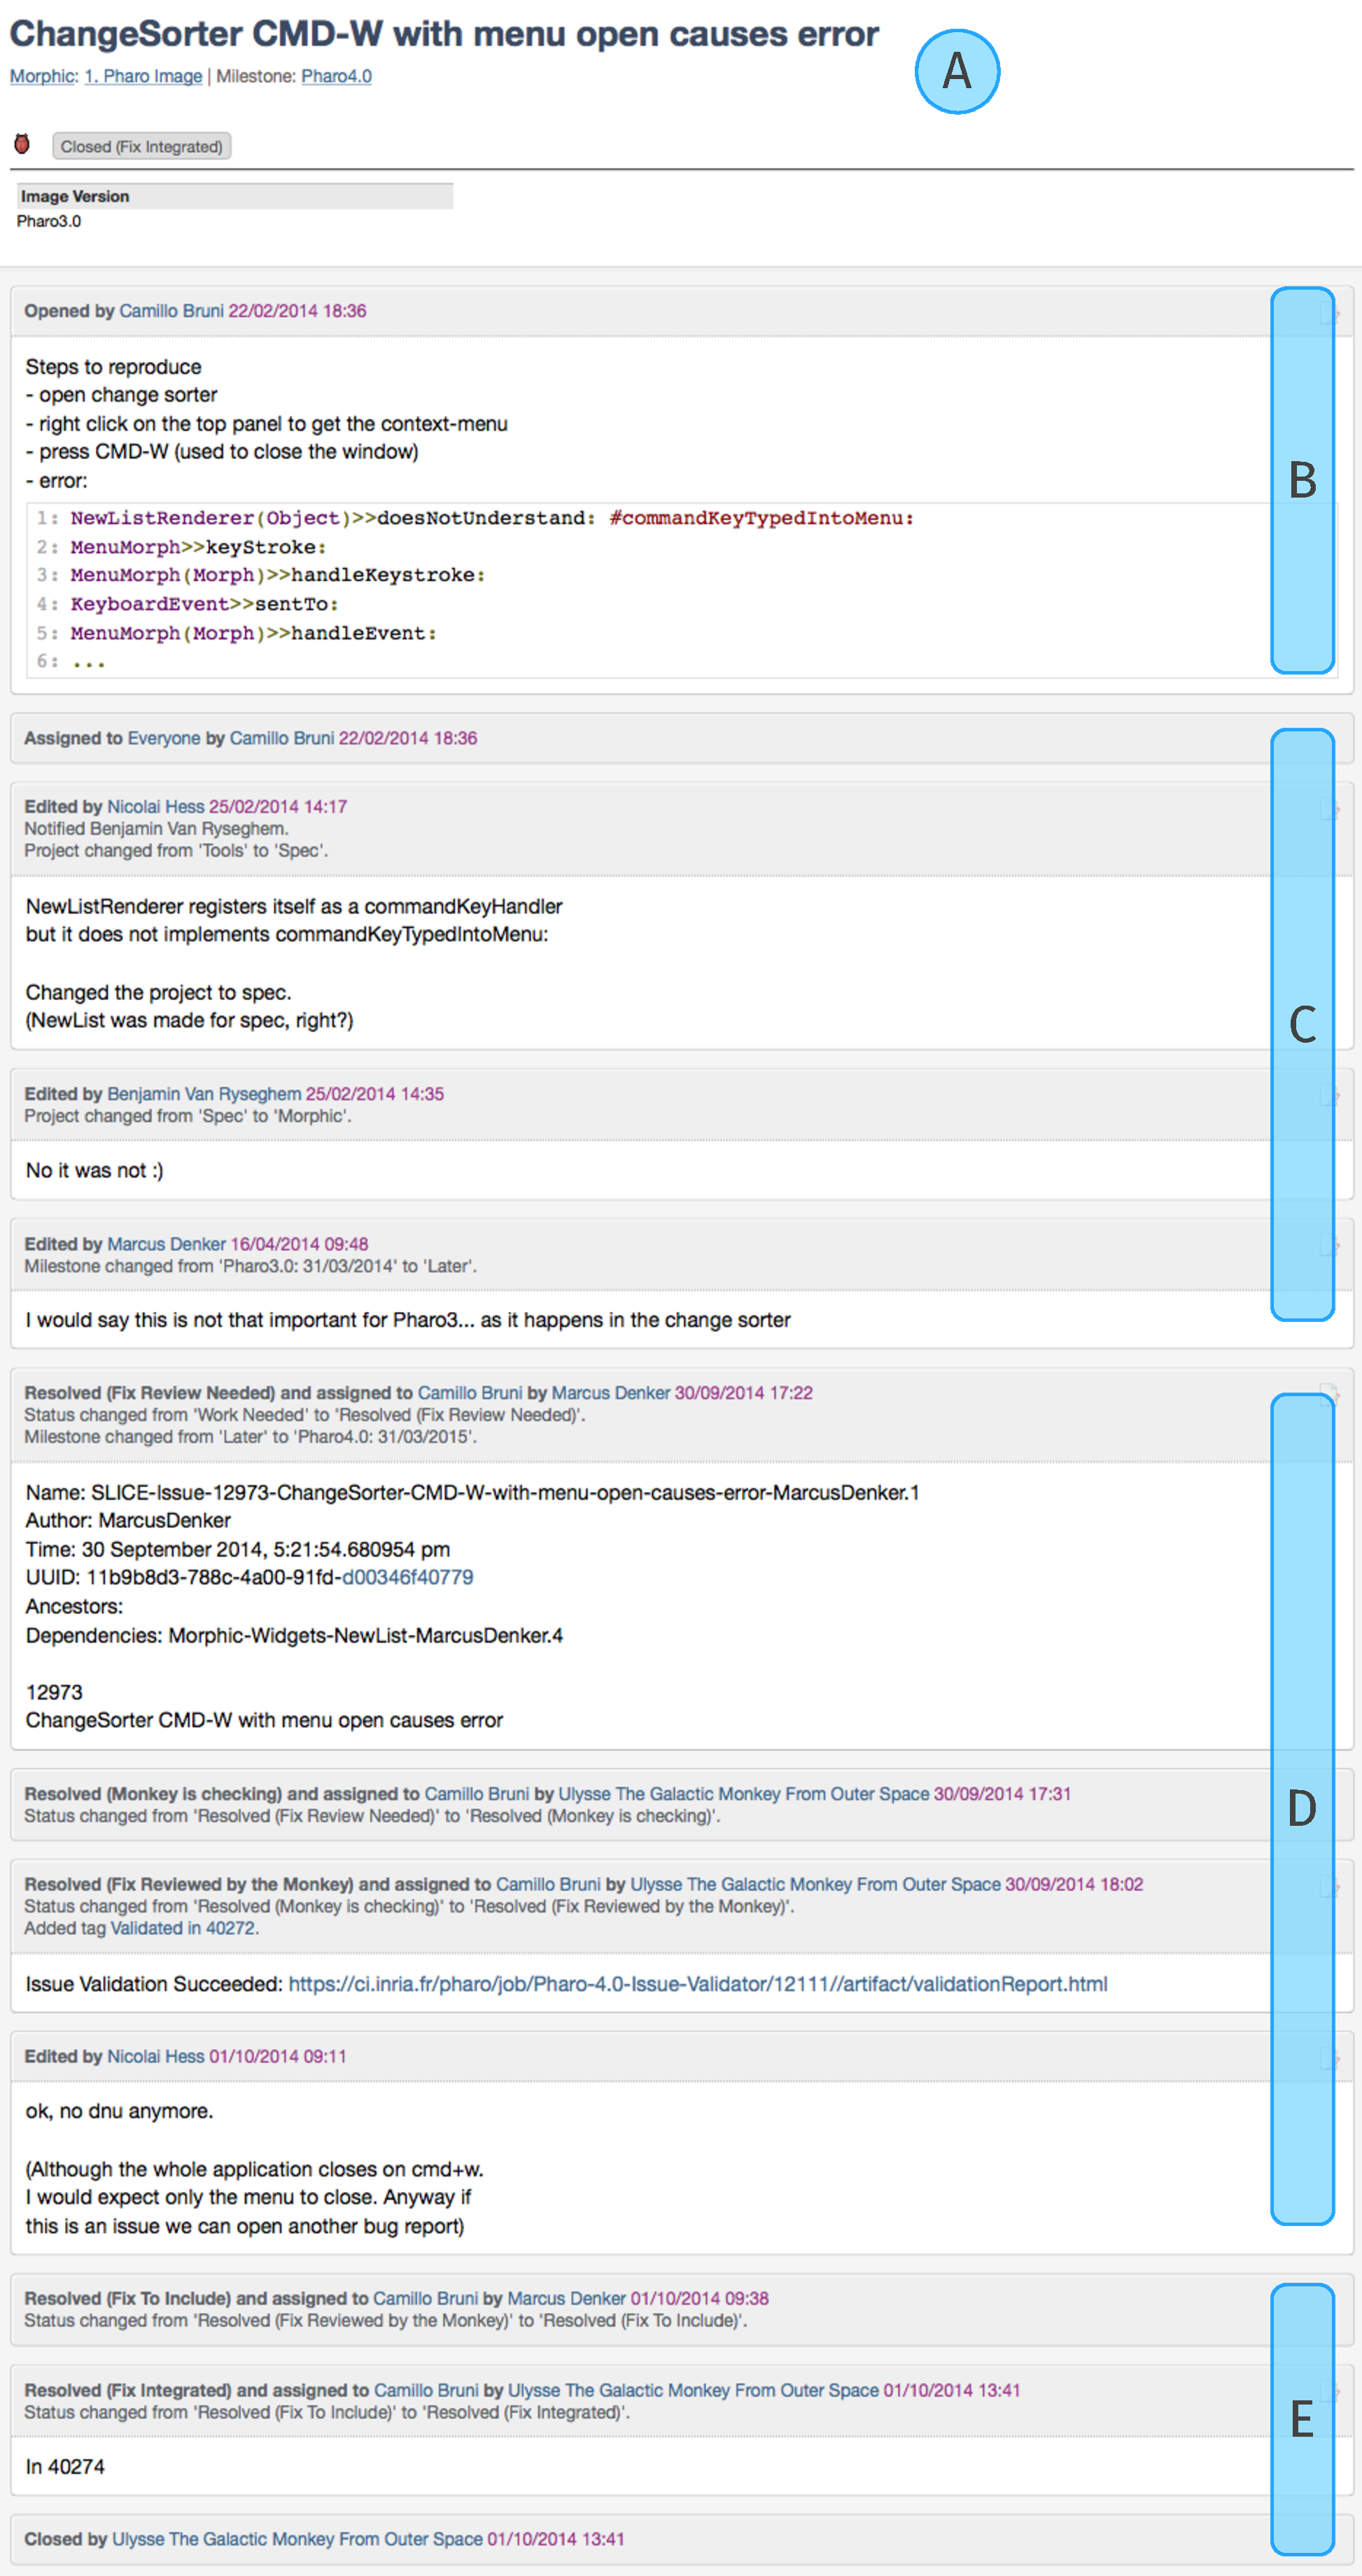
\includegraphics[height=.87\textheight]{stacktraces/Report-12973.pdf}
  \caption{The bug report 12973, related to the stack trace depicted in \figref{fig:stacktrace}.
We can see the metadata (A), the initial description that opened the bug report (B), the discussion that followed (C), the submission of a slice and its validation (D), and the bug resolution (E).}
  \label{fig:report}
\end{center}
\end{figure}

\subsubsection{Example 1}

In \secref{sec:stacktraces-nature} we already presented the stack trace shown in \figref{fig:stacktrace}.
The example is particularly interesting because it shows a practical use case for a user or a developer that encounters the exception while she is writing code.
\figref{fig:report} shows the bug reports retrieved for this stack trace.
As the report shows, there is a known error caused by a defect in the system, and the community is already working to address it.
In particular, since the stack trace that we considered was generated in date 7/7/2014, the user encountered the problem before its resolution and, at the time, the report was stuck in a low priority status.
This information could have been exploited by a developer to report more precise information or to ask for an increase of the priority for a quicker defect resolution, while a user encountering the exception could know that there is work in progress, or if there is an estimated time to have an updated and fixed version.

By continuing to read the report, we can see that the problem has been further investigated, and that a \emph{slice} (a piece of submitted code, that in \pha works in a similar way of a patch) has been proposed and is being tested by the continuous integration server of the project.
Finally we can see that the report was closed, the fix was accepted and it is waiting to be integrated in a later version.

Other than simply useful, this information can improve awareness in the community.
For example, it may disseminate and reward the contributions targeted at improving the general quality of the whole system.


\subsubsection{Example 2} Another example is represented by the stack trace starting with:

{\footnotesize
\begin{center}
\begin{tabular}{l}
SmalllintManifestChecker{>}{>}runRules:onPackage:withoutTestCase: \\
RBPackageEnvironment{>}{>}classesDo: \\
Set{>}{>}do: \\
RBPackageEnvironment{>}{>}classesDo: \\
Set{>}{>}do: \\
RBPackageEnvironment{>}{>}classesDo: \\
SmalllintManifestChecker{>}{>}runRules:onPackage:withoutTestCase: \\
CriticBrowser{>}{>}reapplyRule:
%Set>>do:
%CriticBrowser>>reapplyRule:
%CriticBrowser>>reapplyThisRule
%Array>>do:
%CriticBrowser>>reapplyThisRule
%CriticBrowser>>menu:shifted:
\end{tabular}
\end{center}}


The lines containing \emph{CriticBrowser{>}{>}reapplyRule:} are related to the bug report 14230.
At a closer inspection we can see that the bug report contains only three comments, but the last one points to the report 110473, where a long discussion (40 comments) is ongoing regarding the relation of the method in the stack trace and the application of rules for the CriticBrowser.
At the end of the discussion the report gets closed, but as a result of the fix, another bug report is issued to address further weird behavior of the CodeCriticBrowser.
To add even more correlation to the trace and the report, we noticed that the author of the stack trace is active in the discussion of the report, and actively contributed in its resolution.
This reinforces our belief that providing a bug report context when a user encounters an exception can provide great value in debugging software.




\section{Discussion}\label{sec:stacktraces-discussion}

We discussed our approach and its preliminary results in investigating the stack trace data that we collected.
We now take a critical stance towards our approach, discussing the data, the approach itself and the actual impact that it can have on a development community.


\subsection{The Data}

During this experiment we collected novel data generated from actual daily development activity.
The biggest threat that we see in our work is given by the nature of our dataset.
Despite having a considerable amount of stack traces, the fact that they were produced by just eight developers may introduce hidden patterns caused by the specific style of programming of each developer, or by the codebase the developers were working on during the experiment.
This could lead to a latent bias in our results, that may prove to be too tailored for our users.
We are expanding the number of developers using \slr, and we will therefore be able to verify the generality and scalability of our approach.

Despite this threat, we believe that the data we collected contains valuable and unexploited information, that can lead to the discovery of hidden patterns in developers' activity.
Analyzing this information can produce knowledge that can be helpful in supporting the developers during the bug fixing activities, and can support the work of the community.


\subsection{The Approach}

We designed our approach to find immediate use of the stack traces, and confirm that the data we collected contained information that was both significant and interpretable.
However, there are many improvements that can be done to refine the way that we process stack traces  and link them with bug reports.

One can argue that the use of clustering is not really necessary in finding a correlation between a stack trace and a report, and that a simple direct search of the elements of a stack trace is sufficient to find the relevant matches.
However, we believe that the use of clustering carries some advantages that can be valuable in building a tool to provide feedback on actual data.


\subsubsection{Generalization}
First of all, the use of clustering allows to identify, group and ``average'' similar stack traces, having the effect of making the whole process more robust and noise resistant by considering only the most popular stack trace in the group.
In this way, even changes in the system that would generate different, but still similar stack traces would have no immediate negative impact in the search result.


\subsubsection{Scalability}
Even more important, the use of clustering brings the crucial advantage of drastically reducing the size of the problem.
While this is not an impossible problem to overcome with the size of the dataset that we considered, in a real world scenario with thousands of developer constantly providing stack traces from errors, the volume of the data would quickly become impossible to process.
As such, building clusters that can be used as index and provide a quick lookup for the existing categories of stack traces is a necessary step in building a tool that provides real-time feedback to the user in an acceptable time.


\subsubsection{Metrics}
The final advantage of building clusters is that it eases further analysis on the dataset.
Clustering provides an immediate measure of the popularity of the cluster, it can help in profiling the types of errors on the system during time and ease further investigation on specific groups of stack traces, allowing deeper inspection of other unexpected behaviors on the system, such as the distribution of Message Not Understood or  the distribution of the invoked classes and methods.
To develop this approach, we used a very simple, yet effective clustering method based on the connected components of the graph formed by the nearest neighbor.
Despite its simplicity, this method already provided useful results in identifying the main groups of stack traces in the dataset, as shown in \figref{fig:eva-clusters}.
The approach can be further refined with more specific algorithms, such as k-means~\cite{MacQ1967} or k-medoids~\cite{Kauf1987,Park2009}, which could provide more precise results.
However, the cost for such improvement could be represented by a drop of performance, since these algorithms are computationally expensive.
Therefore, the nearest-neighbor clustering  represents a good tradeoff between results and efficiency.
Also, the problem of a clustering algorithm such as k-means, is that it requires to determine \emph{a priori} the number of clusters to separate our dataset, but in the context of stack traces this information is indeed impossible from the beginning, and it can invalidate the notion of similarity, degrading the approach.
Instead, our approach allows a to define a partition without previous knowledge, and that can be easily an quickly adapted as the number of instances increases, and different classes of exceptions and stack traces are discovered.


\subsection{Applicability of the Method}

We think that the ability to immediately link stack traces to bug reports can be effectively exploited to provide on-line help to a developer.
We foresee additional benefits that require additional investigation and tool support.
Our approach provides quick evidence of the problems in a system and helps finding the immediate context of the error: Therefore, it can be exploited to speed the debugging process, or it can provide information on the current status of a bug in the system.
Moreover, since the information presented to the developer depends on the context she is working on, it may also work as additional documentation, and support the understanding of some parts of the code which are poorly documented.

Besides the pragmatic aspects of assisting developers, we think that having a way to access live information on the status of the system may result in a more integrated and open development process.
A normal user can be reassured by knowing that the core development team is already dealing with a problem, while other developers may be encouraged to step in and help the resolution of the defect, either by providing additional information or by actually start working on the defect.
In an open source project, this set of conditions could bolster the interactions among the community members, focus the attention to current problems and reinforce the whole community.



% \section{Related Work}\label{sec:stacktraces-related}
%
% Bug fixing is well known to be a tedious activity, and identifying the source of a problem---even with a bug report---represents a non trivial task.
% Zimmermann \etal showed that the bug reports containing stack traces improve the general quality of the report, and result in a faster resolution of the report~\cite{Zimm2010a}.
% Schr\"oter \etal provided empirical evidence analyzing the Eclipse project that the use of stack traces in defect resolution provides value in the debugging activity, and suggested that software projects should provide means to include them in defect reporting~\cite{Schr2010a}.
%
% The idea of collecting runtime exceptions to analyze software errors has been adopted by different authors in different contexts.
% Glerum \etal used an automated approach to collect errors generated and submitted by WER, the \emph{Windows Error Reporting} tool.
% They analyzed data collected from users of Microsoft's operating systems worldwide: In their approach approach they grouped the reports into buckets by looking for specific properties of the trace, and used this information to prioritize debugging and build a knowledge base where system administrators could check common problems of the system~\cite{Glerum2009}.
% Inspired by this work, Han Shi~\etal applied the same principle to performance debugging~\cite{Han2012}: They proposed an approach called StackMine, designed to detect and report highly impacting performance bugs and address defects that cause long delays in the user experience.
% We believe that a similar approach to the one that they applied to an operating system, can be a valuable support for developers in building a programming environment.
% Mozilla adopts a similar approach to collect stack traces and runtime execution for debugging purposes~\cite{McLa2004}.
%
% The information of stack traces contained in bug reports represents a valuable support in debugging: as such, many researchers devised different methods to aid bug fixing and management of reports using stack traces.
% These works provided evidence that stack traces are a useful tool and a precious source of information~\cite{Davie2013,Wang2013,Brod2005,Weis2007a}: they provide precise information that are generally more reliable and useful than the descriptions produced by the submitter of the reports~\cite{Ko2006}.
%
% Brodie \etal proposed an automated approach to group similar bug reports using stack trace~\cite{Brod2005}
%
% Moreno \etal applied Text Retrieval techniques to compute similarity between bug reports using the stack traces contained in the report description, focusing on reducing the overhead to analyze large amounts of data~\cite{Moreno2014}.
% Again, this was done in a localized post mortem way.
%
% Managing bug reports is expensive and represents an open problem: Many studies proposed approaches to automatically manage them, by finding the the right developer to fix the defect, predict the cost of fixing a bug and reduce maintenance costs~\cite{Matt2009,Anvi2006a,Sliw2005,DAmb2010c}.
% In this context, we propose an approach to efficiently associate new stack traces to existing bug reports, in an efficient and scalable way, to provide immediate feedback to the users of the system and to assist development and bug fixing in a live fashion.



\section{Outline}\label{sec:stacktraces-summary}
% Wrapping up: http://www.terraceeatery.co.uk/media/catalog/product/cache/1/image/9df78eab33525d08d6e5fb8d27136e95/4/1/415_1.jpg

Fixing defects is an expensive, tedious and time consuming activity: It costs money in industry and it consumes contributors' time---and energy---in open source communities.
The debugging process requires to deeply understand the system, and to gather information to shed light on the nature of the defect.
As a result, the debugging process has the side effect of producing a lot of information describing the context of the error.
This information is however usually discarded after solving the problem.


\subsection{CrowdStacking Traces}

We presented \slr, a tool that seamlessly integrates into the \pha system to collect stack traces produced during the arise of runtime executions in the system.
The goal of \slr is to collect and store information, and reuse it to extract deeper knowledge of the underlying code, assist and boost the whole debugging process.

Given the volume of the data produced by the collection approach, it is crucial to have a way to browse the stored information in an efficient and useful way, that allows fast access to the obtained knowledge.
We presented a study on the data we collected, proposing an approach to group the stack traces into clusters and use those clusters to retrieve useful information for the developers.
We generated the clusters by stack traces similarity, and selected the medoid of each group to represent the archetype of the collection: Each archetype represents a different type of error that happens in the system.
We calculated the popularity of each group, that is determined by the number of stack traces that it contains, and used this metric to rank the clusters.

We showed a possible application to exploit the data contained in stack traces by mining the \pha bug tracker to retrieve the bug reports associated with each archetype of stack trace.
We found a connection with bug reports related to the exception and we showed that the information can be used to aid the debugging activity.
In the cases where the clusters do not have a clear connection with existing bug reports, the system should highlight the anomaly and propose to open a bug report displaying the information gathered until then.

\subsection{Next Steps}

We see this work as first step towards a new way of dealing with information from error contexts.
Current debugging workflows include a number of time consuming activities that could be automated, to reduce the time spent on fixing problems, speed up the development, and foster the improvement of the software project.
The approach that we presented in this chapter is only one of the many possible ways that we see possible to adopt in employing this data: leveraging this information can lead to a number of tools that can deeply impact the way communities and developers deal with debugging.
\begin{itemize}%[$\circ$]
\item\textit{Context aware debugging:} as we suggested during the chapter, we want to extend \slr to propose the possible bug reports to the developer whenever he triggers an exception, to provide a quicker access to the information needed to deal with the problem.

\item\textit{Bug triaging:} Having access to stack trace information can help identifying the types of defects that caused an exception, thus easing the process of triaging the bug~\cite{Anvi2006a}.
Also, we can use the data submitted by each user to create and update profiles of the developers and determine their area of expertise in a quick and reliable way.

\end{itemize}

There still is a significant amount of data that we did not consider during our analysis.
The information regarding the dynamic nature of the language can still be exploited to get insights on the internals of the system.

\begin{itemize}%[$\circ$]

\item\textit{System core exceptions:} We mainly focused on the top part of the trace, because it contains the part of information closer to the user.
The bottom of the stack, which involves the deeper parts of the system, can be used to find bugs hidden in the core classes of the system.

\item\textit{Stack trace patterns:} We saw from \figref{fig:stackcity-classes} and \figref{fig:stackcity-methods} that many stack traces actually touch only a small part of the system.
This is an interesting behavior that we want to investigate further, by looking for patterns in the call stack and detect how to deal with ``hot areas'' of the system.

\item\textit{Optimization:} Knowing the main areas of the system that are executed during an exception can also show the frequency of execution during the daily activity of the users.
This information can be combined with code profiling techniques to determine where and how to perform optimizations on the existing code, and improve execution performances.
\end{itemize}

We envision a future where debugging, but also development activities are supported by means of context-aware tools that use automatically extracted information produced by a whole development community, to aid the tasks of developers and support debugging, with the support of the whole community.


\subsubsection{The Road So Far...}
We have seen how the automatic collection of stack trace generated during a failure can complement the information contained in a bug report with knowledge about the system, to support a number of different debugging and development tasks.
In the next chapter we further push our approach, and generalize it to enable the collection of arbitrary, domain specific data.
